\documentclass[border=10pt]{standalone}
\usepackage{tikz}
\usetikzlibrary{arrows.meta}
\tikzset{%
  >={Latex[width=2mm,length=2mm]},
  % Specifications for style of nodes:
            base/.style = {rectangle, rounded corners, draw=black,
                           minimum width=4cm, minimum height=1cm,
                           text centered, font=\sffamily},
  activityStarts/.style = {base, fill=blue!30},
       startstop/.style = {base, fill=red!30},
    activityRuns/.style = {base, fill=green!30},
         process/.style = {base, minimum width=2.5cm, fill=orange!15},
}
\begin{document}    
% Drawing part, node distance is 1.5 cm and every node
% is prefilled with white background
%\begin{tikzpicture}[node distance=1.5cm,
%    every node/.style={fill=white, font=\sffamily}, align=center]
%  % Specification of nodes (position, etc.)
%  \node (start)             [activityStarts]              {Tudásvezérelt termék};
%  \node (controltech)     [process, below of=start]          {szabályozástechnikai\\problémák};
%  \node (modelbased)      [process, below of=controltech, yshift=-1cm]   {modellalapú irányítás};
%  \node (onResumeBlock)     [process, below of=modelbased]   {onResume()};
%  \node (activityRuns)      [activityRuns, below of=onResumeBlock]
%                                                      {Activity is running};
%  \node (onPauseBlock)      [process, below of=activityRuns, yshift=-1cm]
%                                                                {onPause()};
%  \node (onStopBlock)       [process, below of=onPauseBlock, yshift=-1cm]
%                                                                 {onStop()};
%  \node (onDestroyBlock)    [process, below of=onStopBlock, yshift=-1cm] 
%                                                              {onDestroy()};
%  \node (onRestartBlock)    [process, right of=controltech, xshift=4cm]
%                                                              {onRestart()};
%  \node (ActivityEnds)      [startstop, left of=activityRuns, xshift=-4cm]
%                                                        {Process is killed};
%  \node (ActivityDestroyed) [startstop, below of=onDestroyBlock]
%                                                    {Activity is shut down};     
%  % Specification of lines between nodes specified above
%  % with aditional nodes for description 
%  %\draw[->]            (start) -- (controltech);
%  \draw[->]       (controltech) -- node {MIMO rendszerek, 
%  	                                mérhető zavarások} (modelbased);
%  \draw[->]        (modelbased) -- (onResumeBlock);
%  \draw[->]     (onResumeBlock) -- (activityRuns);
%  \draw[->]      (activityRuns) -- node[text width=4cm]
%                                   {Another activity comes in
%                                    front of the activity} (onPauseBlock);
%  \draw[->]      (onPauseBlock) -- node {The activity is no longer visible}
%                                   (onStopBlock);
%  \draw[->]       (onStopBlock) -- node {The activity is shut down by
%                                   user or system} (onDestroyBlock);
%  \draw[->]    (onRestartBlock) -- (controltech);
%  \draw[->]       (onStopBlock) -| node[yshift=1.25cm, text width=3cm]
%                                   {The activity comes to the foreground}
%                                   (onRestartBlock);
%  \draw[->]    (onDestroyBlock) -- (ActivityDestroyed);
%  \draw[->]      (onPauseBlock) -| node(priorityXMemory)
%                                   {higher priority $\rightarrow$ more memory}
%                                   (ActivityEnds);
%  \draw           (onStopBlock) -| (priorityXMemory);
%  \draw[->]     (ActivityEnds)  |- node [yshift=-2cm, text width=3.1cm]
%                                    {User navigates back to the activity}
%                                    (controltech);
%  \draw[->] (onPauseBlock.east) -- ++(2.6,0) -- ++(0,2) -- ++(0,2) --                
%     node[xshift=1.2cm,yshift=-1.5cm, text width=2.5cm]
%     {The activity comes to the foreground}(onResumeBlock.east);
%  \end{tikzpicture}
%  
  \pagebreak
  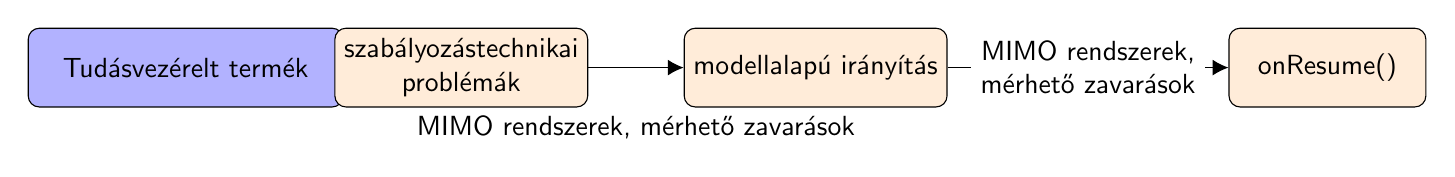
\begin{tikzpicture}[node distance=1.5cm,
  every node/.style={fill=white, font=\sffamily}, align=center]
  
  % Specification of nodes (position, etc.)
  \node (start)           [activityStarts]              {Tudásvezérelt termék};
  \node (controltech)     [process, right of=start, xshift=2cm]          {szabályozástechnikai\\problémák};
  \node (modelbased)      [process, right of=controltech, xshift=3cm]   {modellalapú irányítás};
  \node (onResumeBlock)     [process, right of=modelbased, xshift=5cm]   {onResume()};
%  \node (activityRuns)      [activityRuns, below of=onResumeBlock]
%  {Activity is running};
%  \node (onPauseBlock)      [process, below of=activityRuns, yshift=-1cm]
%  {onPause()};
%  \node (onStopBlock)       [process, below of=onPauseBlock, yshift=-1cm]
%  {onStop()};
%  \node (onDestroyBlock)    [process, below of=onStopBlock, yshift=-1cm] 
%  {onDestroy()};
%  \node (onRestartBlock)    [process, right of=controltech, xshift=4cm]
%  {onRestart()};
%  \node (ActivityEnds)      [startstop, left of=activityRuns, xshift=-4cm]
%  {Process is killed};
%  \node (ActivityDestroyed) [startstop, below of=onDestroyBlock]
%  {Activity is shut down};   
  
    
  % Specification of lines between nodes specified above
  % with aditional nodes for description 
  %\draw[->]            (start) -- (controltech);
  \draw[->]       (controltech) -- node[anchor=north, yshift=-0.5cm] {MIMO rendszerek, 
  	mérhető zavarások} (modelbased);
  \draw[->]        (modelbased) -- node {MIMO rendszerek, \\
  	mérhető zavarások}(onResumeBlock);
%  \draw[->]     (onResumeBlock) -- (activityRuns);
%  \draw[->]      (activityRuns) -- node[text width=4cm]
%  {Another activity comes in
%  	front of the activity} (onPauseBlock);
%  \draw[->]      (onPauseBlock) -- node {The activity is no longer visible}
%  (onStopBlock);
%  \draw[->]       (onStopBlock) -- node {The activity is shut down by
%  	user or system} (onDestroyBlock);
%  \draw[->]    (onRestartBlock) -- (controltech);
%  \draw[->]       (onStopBlock) -| node[yshift=1.25cm, text width=3cm]
%  {The activity comes to the foreground}
%  (onRestartBlock);
%  \draw[->]    (onDestroyBlock) -- (ActivityDestroyed);
%  \draw[->]      (onPauseBlock) -| node(priorityXMemory)
%  {higher priority $\rightarrow$ more memory}
%  (ActivityEnds);
%  \draw           (onStopBlock) -| (priorityXMemory);
%  \draw[->]     (ActivityEnds)  |- node [yshift=-2cm, text width=3.1cm]
%  {User navigates back to the activity}
%  (controltech);
%  \draw[->] (onPauseBlock.east) -- ++(2.6,0) -- ++(0,2) -- ++(0,2) --                
%  node[xshift=1.2cm,yshift=-1.5cm, text width=2.5cm]
%  {The activity comes to the foreground}(onResumeBlock.east);
  \end{tikzpicture}
\end{document}